\documentclass[../main.tex]{subfiles}
\begin{document}
\chapter{Validazione del framework}
In questo capitolo verrà proposta una validazione del lavoro svolto, effettuando una valutazione della sicurezza in un deployment di sviluppo della piattaforma \textit{Moon Cloud}.
L'obiettivo è quello di validare il framework \textit{Moon Cloud} rispetto ai requisiti \textit{FedRAMP}.

A tal fine sono stati effettuati diversi test, ispezionando i livelli \textit{IaaS}, \textit{PaaS} e \textit{SaaS},
eseguendo, ove opportuno, il driver sviluppato in sezione \ref{sec:openscapmooncloud} e presentandone una valutazione delle prestazioni.  

L'ambiente di sviluppo è costituito da un'architettura multi-layer così composta:
\begin{itemize}
    \item A livello di infrastruttura, un nodo fisico, Dell PowerEdge T430 equipaggiato con processore Intel(R) Xeon(R) CPU E5-2630 v4 (10 core fisici e 40 thread logici), 48GB di RAM e 5 dischi da 1TB ciascuno in configurazione RAID 1. Su questa macchina è stato installato il sistema operativo CentOS 7.2, e il software OpenStack Newton.

        È stata quindi effettuata la valutazione della sicurezza a livelli di sistema operativo, utilizzando il driver \textit{OpenSCAP} (del quale sono state collezionate alcune misurazioni sull'impatto prestazionale), e successivamente è stato proposto un benchmarking del setup OpenStack, effettuando un mapping delle recommendation descritte dell'articolo \textit{"A security benchmark for OpenStack"}\cite{MyPaper} sui \textit{security control} FedRAMP.
    \item A livello di piattaforma, un cluster Docker Swarm composto da 3 macchine virtuali identiche, con 4GB di RAM, 10GB di disco e sistema operativo CentOS 7.2.
        
        La valutazione della sicurezza è stata effettuata tramite il driver \textit{OpenSCAP} per analizzare il sistema operativo \textit{guest}, poi eseguendo il \textit{Docker Benchmark for Security}\footnote{https://dockerbench.com} proponendo, anche in questo caso, il mapping tra i risultati ottenuti e i \textit{requisiti FedRAMP}.
        \vfill\newpage

    \item A livello applicativo, i componenti di Moon Cloud: 5 microservizi \textit{core} e 2 microservizi per la gestione del nodo di esecuzione.\\
        \textbf{Componenti Core}
        \begin{itemize}
            \item API
            \item Database
            \item Repository
            \item Database dei risultati
            \item Evaluation Manager
        \end{itemize}
        \textbf{Componenti execution node e execution cluster}
        \begin{itemize}
            \item Execution Manager
            \item Reverse proxy
        \end{itemize}

        È stato effettuato l'\textit{assessment} dei vari componenti di \textit{Moon Cloud} e dei meccanismi di integrazione e comunicazione utilizzati; per ragioni di proprietà intellettuale, l'analisi è stata illustrata ad alto livello.
\end{itemize}

\section{Infrastruttura}
La valutazione dei componenti infrastrutturali si è svolta in due fasi:
\begin{enumerate}
    \item Assessment del sistema operativo del server fisico, utilizzando il driver \textit{OpenSCAP} illustrato in sezione \ref{sec:openscapmooncloud}, del quale sono state collezionate informazioni sulle performance di esecuzione;
    \item Valutazione di OpenStack sulla base deile recommendation dell'articolo \textit{"A security benchmark for OpenStack"}\cite{MyPaper}. 
\end{enumerate}

\subsection{Analisi OpenSCAP del server fisico}
\begin{comment}
test finished
started at 1496183480
ended at   1496184352
lasted -872 seconds
report available at
https://moonclouddashboard.blob.core.windows.net/pdfcontainer/f4a1943cff
Il test è stato eseguito utilizzando il driver realizzato, specificando in input il documento XCCDF "\textit{ssg-centos7}" unitamente al profilo "\textit{nist-800-171-cui}". 
\end{comment}
Per il primo test eseguito, è stato utilizzato il driver realizzato, il quale effettua una connessione SSH al sistema target, verifica che sia installato \textit{OpenSCAP}, effettua il caricamento dei file XCCDF selezionati, e ne esegue l'assessment caricando poi i risultati sul servizio di storage di oggetti di Microsoft Azure.

Il documento \textit{JSON} dato in input al test è il seguente:
\begin{js}
{
    "read_ssh_configuration": {
    },
    "read_xccdf_configuration": {
        "xccdf":"ssg-centos7",
        "profile":"nist-800-171-cui",
        "fetch_remote_resources": true
    },
    "read_azure_configuration": {
    }
}
\end{js}
La sezione \textit{read\_ssh\_configuration} contiene i parametri per la connessione SSH, che sono stati omessi per motivi di riservatezza; in \textit{read\_xccdf\_configuration}, sono invece specificati:
\begin{itemize}
    \item Il documento XCCDF (\textit{ssg-centos7}), contenente la checklist automatizzabile da eseguire
    \item Il profilo (\textit{nist-800-171-cui}), che specifica i test effettivamente selezionati per l'esecuzione (il profilo in questione, sebbene di valore semantico apparentemente differente da quanto atteso, include i test \textit{NIST 800-53}).
    \item La volontà di effettuare il download delle risorse remote specificate nella checklist.
\end{itemize}
Infine, \textit{read\_azure\_configuration} contiene i parametri per l'upload del report su Microsoft Azure, anch'essi omessi per ragioni di riservatezza.

L'esecuzione del test ha riportato:
\begin{itemize}
    \item 119 valutazioni effettuate con successo
    \item 72 valutazioni fallite
\end{itemize}
\begin{figure}[H]
    \centering
    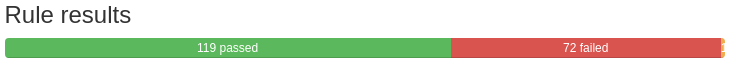
\includegraphics[width=15cm]{immagini/test_oscap_1.png}
\end{figure}

In particolare, delle 72 valutazioni fallite, 11 sono state catalogate da OpenSCAP con \textit{severity} bassa, 50 con \textit{severity} media e 11 con \textit{severity} elevata; lo score della copertura XCCDF ottenuto è 71.17\%.
\subsubsection{Risultato del test: valutazioni fallite}
\begin{ltabulary}{|p{10cm}|p{4cm}|}
    \hline
    \textbf{Descrizione} & \textbf{Security Control}
    \\ \hline
    \endhead

Allow Only SSH Protocol 2                                                             & AC-17, IA-5 \\ \hline
Build and Test AIDE Database                                                          & CM-3(d), CM-3(e), CM-6(d), CM-6(3), SC-28, SI-7 \\ \hline
Configure AIDE to Use FIPS 140-2 for Validating Hashes                                & SI-7(1) \\ \hline
Configure AIDE to Verify Access Control Lists (ACLs)                                  & SI-7.1 \\ \hline
Configure AIDE to Verify Extended Attributes                                          & SI-7.1 \\ \hline
Configure Notification of Post-AIDE Scan Details                                      & CM-3(5)  \\ \hline
Configure Periodic Execution of AIDE                                                  & CM-3(d), CM-3(e), CM-3(5), CM-6(d), CM-6(3), SC-28, SI-7 \\ \hline
Configure the root Account for failed Password Attempts                               & AC-7(b) \\ \hline
Direct root Logins Not Allowed                                                        & IA-2(1) \\ \hline
Disable Compression Or Set Compression to delayed                                     & CM-6(b) \\ \hline
Disable Ctrl-Alt-Del Reboot Activation                                                & AC-6 \\ \hline
Disable GSSAPI Authentication                                                         & CM-6(c) \\ \hline
Disable KDump Kernel Crash Analyzer (kdump)                                           & AC-17(8), CM-7, CM-6(b) \\ \hline
Disable Kerberos Authentication                                                       & CM-6(c) \\ \hline
Disable Prelinking                                                                    & CM-6(c) \\ \hline
Disable SSH Access via Empty Passwords                                                & AC-3, AC-6, CM-6(b) \\ \hline
Disable SSH Root Login                                                                & AC-3, AC-17(2), AU-10(5), CM-6(b), IA-5(1)(c), IA-7 \\ \hline
Disable SSH Support for Rhosts RSA Authentication                                     & AC-3, AC-6, CM-6(b) \\ \hline
Disable SSH Support for User Known Hosts                                              & CM-6(a) \\ \hline
Disable Support for RPC IPv6                                                          & CM-6(a) \\ \hline
Disable xinetd Service                                                                & AC-17(8), CM-7 \\ \hline
Do Not Allow SSH Environment Options                                                  & CM-6(b)  \\ \hline
Enable Smart Card Login                                                               & IA-2(2) \\ \hline
Enable SSH Warning Banner                                                             & AC-8(a), AC-8(b), AC-8(c)(1), AC-8(c)(2), AC-8(c)(3) \\ \hline
Enable Use of Privilege Separation                                                    & AC-6 \\ \hline
Enable Use of Strict Mode Checking                                                    & AC-6 \\ \hline
Ensure gpgcheck Enabled For All Yum Package Repositories                              & CM-5(3), SI-7, MA-1(b) \\ \hline
Ensure gpgcheck Enabled for Local Packages                                            & CM-5(3) \\ \hline
Ensure gpgcheck Enabled for Repository Metadata                                       & CM-5(3) \\ \hline
Ensure Logs Sent To Remote Host                                                       & AU-3(2), AU-4(1), AU-9 \\ \hline
Ensure System is Not Acting as a Network Sniffer                                      & CM-7, CM-7(2).1(i) \\ \hline
Ensure the Logon ure Delay is Set Correctly in login.defs                             & IA-5(f), IA-5(1)(a) \\ \hline
Ensure YUM Removes Previous Package Versions                                          & SI-2 \\ \hline
Install AIDE                                                                          & CM-3(d), CM-3(e), CM-6(d), CM-6(3), SC-28, SI-7 \\ \hline
Install the dracut-fips Package                                                       & AC-17(2) \\ \hline
Install Virus Scanning Software                                                       & SC-28, SI-3 \\ \hline
Limit Password Reuse                                                                  & IA-5(1)(e) \\ \hline
Limit the Number of Concurrent Login Sessions Allowed Per User                        & AC-10  \\ \hline
Modify the System Login Banner                                                        & AC-8(a), AC-8(b), AC-8(c)(1), AC-8(c)(2), AC-8(c)(3) \\ \hline %
Prevent Log In to Accounts With Empty Password                                        & AC-6, IA-5(b), IA-5(c), IA-5(1)(a) \\ \hline
Restrict Serial Port Root Logins                                                      & AC-6(2) \\ \hline
Restrict Virtual Console Root Logins                                                  & AC-6(2) \\ \hline
Set Account Expiration Foling Inactivity                                              & AC-2(2), AC-2(3), IA-4(e) \\ \hline
Set Deny For failed Password Attempts                                                 & AC-7(b) \\ \hline
Set Interactive Session Timeout                                                       & AC-12, SC-10 \\ \hline
Set Interval For Counting ed Password Attempts                                        & AC-7(b) \\ \hline
Set Lockout Time For ed Password Attempts                                             & AC-7(b) \\ \hline
Set Password Maximum Age                                                              & IA-5(b), IA-5(c), IA-5(1)(a) \\ \hline
Set Password Maximum Consecutive Repeating Characters                                 & IA-5(b), IA-5(c), IA-5(1)(a) \\ \hline
Set Password Minimum Age                                                              & IA-5(b), IA-5(c), IA-5(1)(a) \\ \hline
Set Password Minimum Length                                                           & IA-5(b), IA-5(c), IA-5(1)(a) \\ \hline
Set Password Minimum Length in login.defs                                             & IA-5(b), IA-5(c), IA-5(1)(a) \\ \hline
Set Password Retry Prompts Permitted PSession                                         & IA-5(b), IA-5(c), IA-5(1)(a) \\ \hline
Set Password Strength Minimum Different Categories                                    & IA-5(b), IA-5(c), IA-5(1)(a) \\ \hline
Set Password Strength Minimum Different Characters                                    & IA-5(b), IA-5(c), IA-5(1)(a) \\ \hline
Set Password Strength Minimum Digit Characters                                        & IA-5(b), IA-5(c), IA-5(1)(a) \\ \hline
Set Password Strength Minimum Special Characters                                      & IA-5(b), IA-5(c), IA-5(1)(a) \\ \hline
Set Password Strength Minimum Uppercase Characters                                    & IA-5(b), IA-5(c), IA-5(1)(a) \\ \hline
Set Password to Maximum of Consecutive Repeating Characters from Same Character Class & IA-5(b), IA-5(c), IA-5(1)(a) \\ \hline
Set SSH Client Alive Count                                                            & AC-2(5), SA-8, AC-12 \\ \hline
Set SSH Idle Timeout Interval                                                         & AC-7(b) \\ \hline
The Installed Operating System Is Vendor Supported and Certified                      & SI-2(c) \\ \hline
Uninstall xinetd Package                                                              & AC-17(8), CM-7 \\ \hline
Use Only FIPS 140-2 Validated Ciphers                                                 & AC-3, AC-17(2), AU-10(5), CM-6(b), IA-5(1)(c), IA-7 \\ \hline
Use Only FIPS 140-2 Validated MACs                                                    & AC-17(2), IA-7, SC-13 \\ \hline
Verify and Correct File Permissions with RPM                                          & AC-6, AU-9(1), AU-9(3), CM-6(d), CM-6(3) \\ \hline
Verify File Hashes with RPM                                                           & CM-6(d), CM-6(3), SI-7(1) \\ \hline
Verify firewalld Enabled                                                              & CM-6(b) \\ \hline

\end{ltabulary}
\captionof{table}{Risultati valutazione driver OpenSCAP a livello IaaS} 
\begin{figure}[H]
    \centering
    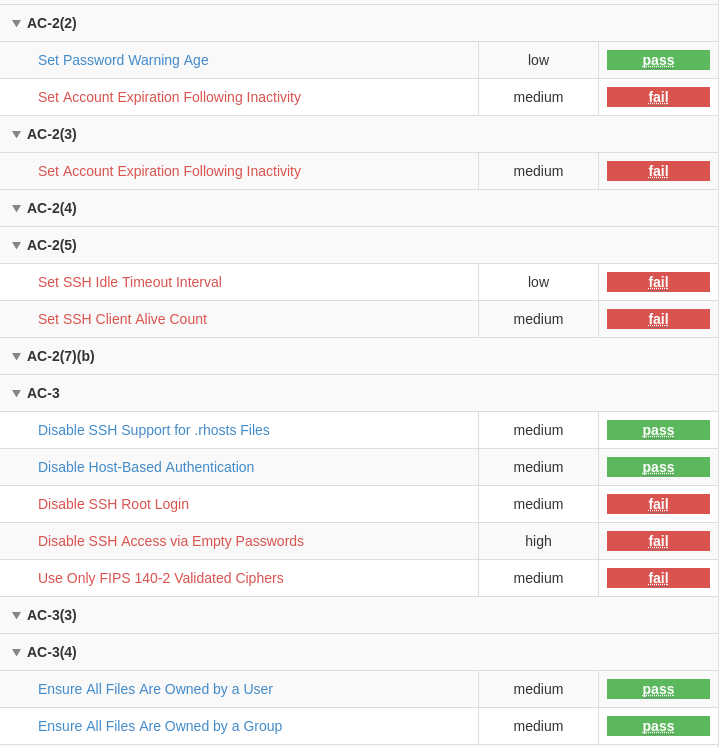
\includegraphics[width=10cm]{immagini/test_oscap_1_1.png}
    \caption{Estratto del report}\label{ref:report_oscap_1_1}
\end{figure}
    
In figura \ref{ref:report_oscap_1_1} è riportata una parte del report generato dal controllo sviluppato. Esso, in formato HTML, contiene il riepilogo di tutti i test eseguiti con il relativo stato e gli script di \textit{remediation}. Il documento completo è disponibile in formato HTML all'indirizzo:\\
\textit{https://moonclouddashboard.blob.core.windows.net/pdfcontainer/f4a1943cff}
\\
o nel repository GIT\\
\textit{https://github.com/patriziotufarolo/tesi\_magistrale/}.


Relativamente all'analisi condotta a livello infrastruttura e stata effettuata 	un'analisi delle performance e del costo dell'esecuzione del driver OpenSCAP.

La valutazione delle \textit{OVAL} mediante il driver realizzato è durata 872 secondi; di seguito sono riportate le statistiche relative all'utilizzo delle risorse nell'esecuzione del test.
Queste sono state raccolte tramite il software \texttt{pidstat}, isolando esclusivamente i processi coinvolti nel processo di assessment.
\begin{figure}[H]
 \begin{minipage}[b]{6cm}
   \centering
   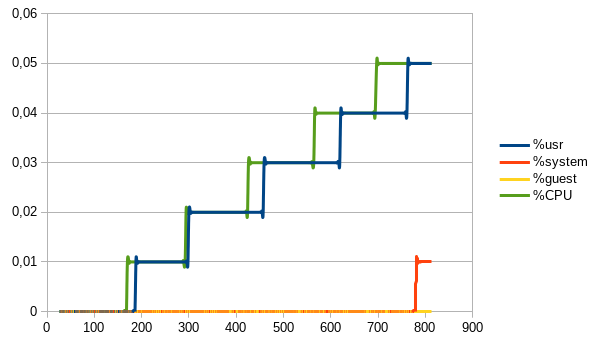
\includegraphics[width=6.6cm]{immagini/plot1cpu.png}
 \end{minipage}
 \hspace{2mm} \hspace{3mm}
 \begin{minipage}[b]{9cm}
  \centering
   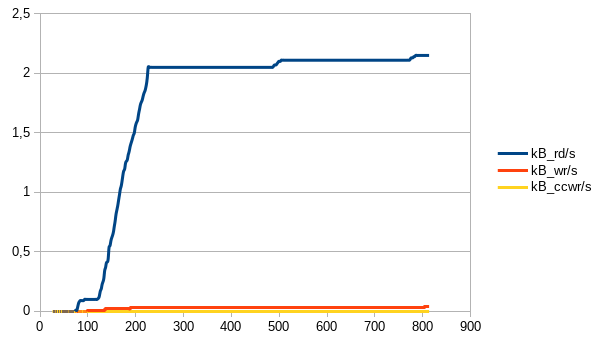
\includegraphics[width=6.6cm]{immagini/plot1io.png}
 \end{minipage}
 \caption{Utilizzo della CPU e carico IO}\label{ref:plot1cpuio}
\end{figure}
Dalla figura \ref{ref:plot1cpuio} è possibile notare come l'impatto del test sulle prestazioni del target sia minimo, registrando picchi di carico sulla CPU inferiori all'0.06\% per tutta la durata dell'esecuzione. Anche dal punto di vista delle operazioni di input/output il test si è dimostrato assolutamente non invasivo, registrando picchi in lettura di pochi KB. 
\begin{figure}[H]
 \begin{minipage}[b]{6cm}
   \centering
   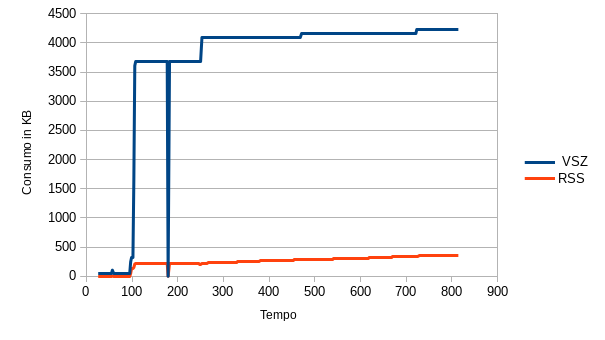
\includegraphics[width=6.6cm]{immagini/plot1mem.png}
 \end{minipage}
 \hspace{2mm} \hspace{3mm}
 \begin{minipage}[b]{9cm}
  \centering
   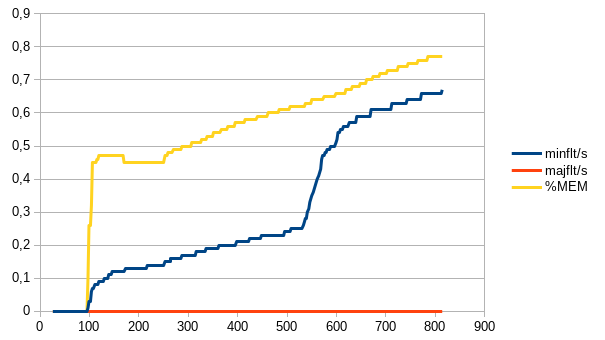
\includegraphics[width=6.6cm]{immagini/plot1mem2.png}
 \end{minipage}
 \caption{Utilizzo della memoria}\label{ref:plot1mem}
\end{figure}
In figura \ref{ref:plot1mem} è stato invece illustrato l'utilizzo della memoria durante l'esecuzione del test, che rimane sempre inferiore all'1\%. Anche in questo caso l'impatto prestazionale è minimo; il \textit{footprint} di \textit{OpenSCAP} e delle relative \textit{probes} non raggiunge i 5MB in memoria virtuale (\textit{VSZ}), rimanendo inoltre sotto i 500 KB in memoria RAM(\textit{RSS}).

Questo driver si presta particolarmente a scenari di esecuzione programmata e automatica, per effettuare monitoraggio continuativo, dimostrandosi adeguato per l'utilizzo in Moon Cloud, il cui obiettivo è quello di effettuare controlli periodici per la valutazione della compliance.
Come discusso nel Capitolo 3, FedRAMP fornisce un programma di autorizzazione ciclico, le cui attività sono svolte da organizzazioni eterogenee con periodicità generalmente semestrali o annuali. L'utilizzo di strumenti di monitoraggio continuativo ed auditing è demandato al \textit{cloud service provider} ed alle organizzazioni di terze parti ingaggiate; in relazione alle analisi di performance svolte ed alla completezza dei risultati ottenibili mediante \textit{OpenSCAP}, è possibile affermare che il driver sviluppato abilita Moon Cloud a diventare uno strumento di supporto per le attività del CSP e delle 3PAO.

\subsection{Analisi di OpenStack}
I documenti XCCDF forniti da OpenSCAP non sono risultati efficienti per l'assessment dei controlli di sicurezza per OpenStack, in quanto le definizioni \textit{OVAL} non sono state completate.

Questa sezione, pertanto, fa riferimento ad alcune raccomandazioni del paper "\textit{A Security Benchmark for OpenStack}" \cite{MyPaper}. Ogni raccomandazione recensita è mappata sui requisiti FedRAMP corrispondenti. A causa del fatto che l'implementazione dei controlli automatici per alcuni di queste non sono disponibili, l'analisi è stata fatta in modo manuale ispezionando le configurazioni.

Laddove è applicata la dicitura "Non applicabile", si intende che il controllo non è effettuabile nello specifico scenario valutato.
\begin{ltabulary}{|p{6cm}|p{4cm}|p{2cm}|}
    \hline
    \textbf{Reccomendation} & \textbf{FedRAMP SCs} & \textbf{Risultato} \\ \hline
    \endhead 
    {[R1]} Patch Levels                                                                              &  CM-2, CM-2(2), SA-10(1), SI(3)                  & Passato         \\ \hline
    {[R2]} Create and Enforce Account and Password Management Policies                                & AC-2, AC-2(3), AC-6, AC-7, AC-9  & Fallito         \\ \hline
    {[R3]} Use a Central Directory for Authentication and Authorization.                              & AC-3, AC-17                      & Fallito         \\ \hline
    {[R4]} Configure Firewalls to Restrict Access                                                     & CM-6, CM-7                       & Passato         \\ \hline
    {[R5]} Use TLS/SSL where Possible                                                                 & AC-3, AC-17(2), AU-10(5), CM-6(b), IA-5(1)(c), IA-7 & Fallito  \\ \hline
    {[R6]} Do Not Use Default Self-Signed Certificates.                                               & AC-3, AC-17(2), AU-10(5), CM-6(b), IA-5(1)(c), IA-7 & Non Applicabile \\ \hline
    {[R7]} Configure Centralized Remote Logging                                                       & AU-3(2), AU-4(1), AU-9           & Fallito         \\ \hline
    {[R8]} Maintain Time Synchronization Services                                                     & AU-8                             & Passato         \\ \hline
    {[R11]} Use Templates to Deploy Virtual Machines                                                  & -                                & Passato         \\ \hline
    {[R13]} Disable MAC Address Changes and Promiscuous Mode on Guests                                & CM-7, CM-7(2).1(i)               & Passato         \\ \hline
    {[R14]} Ensure Network Isolation through VLANs                                                    & SC-2, SC-7, SC-8                 & Passato         \\ \hline
    {[R15]} Port Groups Should not be Configured to Reserved VLANs                                    & CM-7                                & Passato         \\ \hline
    {[R16]} Secure Access to Cloud Application Programming Interfaces                                 & CM-7                                & Fallito         \\ \hline
    {[R17]} Encrypt Data at Rest                                                                      & SC-28, SC-28 (1)                & Fallito         \\ \hline
    {[R18]} Establish Appropriate Resource Isolation                                                  & SC-39                           & Passato         \\ \hline
    {[R19]} Evaluate Denial of Service Scenarios and Mitigations                                      & SC-06                            & Fallito         \\ \hline
    {[R20]} Do Not Use or Set Guest Customization Passwords                                           & IA-5(7)                          & Passato         \\ \hline
    {[R22]} Audit Sensible and Configuration Files                                                    & AU-3, AU-8, AU-12                & Fallito         \\ \hline
    {[R23]} Storage Reliability                                                                       & CP-4, CP-9                       & Fallito         \\ \hline
    {[R24]} Data Remanence Avoidance                                                                  & SC-4                             & Fallito         \\ \hline
\end{ltabulary}
\begin{center}
\captionof{table}{Valutazione della compliance FedRAMP nel setup OpenStack di Moon Cloud} 
\label{table:fedr_os}
\end{center}

In Tabella \ref{table:fedr_os}, è possibile vedere come il 55\% delle valutazioni abbia avuto esito negativo su questo setup OpenStack, in quanto esso non è predisposto per essere utilizzato in scenari di produzione.

\section{Piattaforma}
La valutazione della sicurezza è stata effettuata tramite il driver \textit{OpenSCAP} per analizzare il sistema operativo \textit{guest}, poi eseguendo il \textit{Docker Benchmark for Security}\footnote{https://dockerbench.com} proponendo, anche in questo caso, il mapping tra i risultati ottenuti e i \textit{requisiti FedRAMP}.

\subsection{Analisi OpenSCAP sul template delle macchine virtuali}
Il test con il driver OpenSCAP è stato ripetuto sulle macchine virtuali dei nodi appartenenti al cluster Swarm.

I risultati restituiti in output segnalano:
\begin{itemize}
    \item 122 valutazioni effettuate con successo
    \item 69 valutazioni fallite
\end{itemize}
\begin{figure}[H]
    \centering
    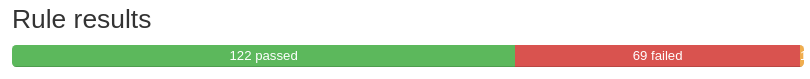
\includegraphics[width=15cm]{immagini/test_oscap_2.png}
\end{figure}

Il report completo è disponibile all'indirizzo \\
\textit{https://moonclouddashboard.blob.core.windows.net/pdfcontainer/b73210ae24}    \\   
oppure \\
\textit{https://www.github.com/patriziotufarolo/tesi\_magistrale/} \\


\begin{comment}
test finished
started at 1496218136
ended at 1496218350
lasted -214 seconds

report available at
https://moonclouddashboard.blob.core.windows.net/pdfcontainer/b73210ae24
--
\end{comment}
\subsection{Analisi del cluster Docker Swarm}
\label{ref:dockerswarmanalysis}
L'analisi del cluster Swarm è stata condotta utilizzando lo strumento \textit{Docker Security Benchmark}\footnote{Docker Security Benchmark - \textit{https://www.dockerbench.com}}.
Poiché i nodi del cluster sono stati creati a partire dallo stesso template, è proposta di seguito un'unica analisi.
Di seguito è proposto un mapping tra le verifiche fallite e i controlli di sicurezza FedRAMP non rispettati; per motivi di proprietà intellettuale i nomi di alcuni container sono stati oscurati.

    \begin{ltabulary}{|p{9cm}|p{5cm}|}
        \hline
        \textbf{Controllo} & \textbf{FedRAMP SCs} \\
        \hline
        \endhead

Audit docker daemon - /usr/bin/docker                                                                                                                                                                                                                                                       & AU-3, AU-8, AU-12                                   \\ \hline
Audit Docker files and directories - /var/lib/docker, /etc/docker, docker.service, /docker-containerd, docker-runc                                                                                                                                                                          & AU-3, AU-8, AU-12                                   \\ \hline
Restrict network traffic between containers                                                                                                                                                                                                                                                 & SC-2, SC-7, SC-8                                    \\ \hline
Docker daemon currently listening on TCP without TLS                                                                                                                                                                                                                                        & AC-3, AC-17(2), AU-10(5), CM-6(b), IA-5(1)(c), IA-7 \\ \hline
Enable user namespace support                                                                                                                                                                                                                                                               & AC-4(21), AC-5, AC-6 (01), AC-6(02), AC-6(05)       \\ \hline
Use authorization plugin                                                                                                                                                                                                                                                                    & AC-3 AC-4                                                    \\ \hline
Configure centralized and remote logging                                                                                                                                                                                                                                                    & AU-3(2), AU-4(1), AU-9                           \\ \hline
Disable operations on legacy registry (v1)                                                                                                                                                                                                                                                  & -                                                 \\ \hline
Bind swarm services to a specific host interface                                                                                                                                                                                                                                            & SC-2, SC-7, SC-8, SC-10                                                     \\ \hline
Unencrypted overlay network: ingress (swarm), mooncloud (swarm)                                                                                                                                                                                                                             & SC-8, SC-8(1), SC-10                                                     \\ \hline
Run swarm manager in auto-lock mode                                                                                                                                                                                                                                                         & SC-27                                               \\ \hline
Create a user for the container                                                                                                                                                                                                                                                             &  AC-4(21), AC-5, AC-6 (01), AC-6(02), AC-6(05)                                                     \\ \hline
Running as root:  mooncloud\_evaluationmodule, mooncloud\_api, mooncloud\_traefik, mooncloud\_monitor\_execution\_manager, mooncloud\_dashboard, mooncloud\_*********, mooncloud\_***********, mooncloud\_db, mooncloud\_******, mooncloud\_execution\_manager                              &  AC-4(21), AC-5, AC-6 (01), AC-6(02), AC-6(05)                                                   \\ \hline
Enable Content trust for Docker:  mooncloud\_evaluationmodule, mooncloud\_api, mooncloud\_traefik, mooncloud\_monitor\_execution\_manager, mooncloud\_dashboard, mooncloud\_*********, mooncloud\_***********, mooncloud\_db, mooncloud\_******, mooncloud\_execution\_manager              &  AU-3(1), CM-07, SC-07, SC-08                                                   \\ \hline
No AppArmorProfile Found:   mooncloud\_evaluationmodule, mooncloud\_api, mooncloud\_traefik, mooncloud\_monitor\_execution\_manager, mooncloud\_dashboard, mooncloud\_*********, mooncloud\_***********, mooncloud\_db, mooncloud\_******, mooncloud\_execution\_manager                    & AC-3, AC-4, AC-5, AC-6, AU-5                    \\ \hline
No selinux SecurityOptions Found:  mooncloud\_evaluationmodule, mooncloud\_api, mooncloud\_traefik, mooncloud\_monitor\_execution\_manager, mooncloud\_dashboard, mooncloud\_*********, mooncloud\_***********, mooncloud\_db, mooncloud\_******, mooncloud\_execution\_manager             & AC-3, AC-4, AC-5, AC-6, AU-5                      \\ \hline
Container running with root FS mounted R/W:  mooncloud\_evaluationmodule, mooncloud\_api, mooncloud\_traefik, mooncloud\_monitor\_execution\_manager, mooncloud\_dashboard, mooncloud\_*********, mooncloud\_***********, mooncloud\_db, mooncloud\_******, mooncloud\_execution\_manager   & SI-12                                           \\ \hline
%SA-2
\end{ltabulary}

Dall'analisi è emerso che non sono stati installati meccanismi di auditing, né per il demone Docker, né per i relativi file di configurazione, inoltre le attività di logging non avvengono in modo centralizzato. Ciò viola i requisiti FedRAMP appartenenti alla classe auditing, in particolar modo \textit{AU-3}, \textit{AU-8} e \textit{AU-12}.
Il demone Docker è in ascolto su una porta TCP (piuttosto che su una socket Unix), senza che la crittografia \textit{TLS} sia stata abilitata;  Il kernel, inoltre, non è stato compilato con il supporto ai \textit{namespace utente}, il cui obiettivo è quello di isolare ulteriormente le attività del container, né è stato creato un utente specifico per ciascun servizio; il filesystem dei container non viene montato in modalità read-only.
Per le reti di overlay, inoltre, non è stata abilitata la crittografia (in violazione di \textit{SC-8}, \textit{SC-8(1)}, \textit{SC-10}): l'onere di proteggere le comunicazioni è lasciato al livello \textit{SaaS}.
Infine, non sono stati abilitati software di mandatory access control come SELinux e AppArmor (in violazione di \textit{AC-3}, \textit{AC-4}, \textit{AC-5}, \textit{AC-6}, \textit{AU-5}).
\section{Livello applicativo: analisi dei microservizi}

L'attività di assessment a livello applicativo è stata svolta ispezionando le configurazioni dei servizi e la loro implementazione, in un ambiente di sviluppo.
Per ragioni di proprietà intellettuale sarà di seguito fornita una descrizione ad alto livello dei componenti e delle problematiche individuate.

\begin{ltabulary}{|p{3cm}|p{11cm}|}
\hline
\textbf{Componente} & \textbf{Analisi} \\
\hline
\endhead

API e Database & È stato effettuato un \textit{vulnerability assessment} blackbox sfruttando i software \textit{SQLMap}\footnote{SQLMap, \textit{http://www.sqlmap.org}} e \textit{OpenVAS}\footnote{OpenVAS, \textit{http://www.openvas.org}} e non sono state riscontrate vulnerabilità note.
Le API sono esposte con protocollo \textit{HTTPS}, il certificato ha chiave \textit{RSA} a 4096 bit, è firmato con \textit{SHA256} ed è stato emesso dalla Certification Authority \textit{Let's Encrypt Authority X3}. Sono supportati i protocolli \textit{TLSv1}, \textit{TLSv1.1}, \textit{TLSv1.2}, il supporto a \textit{SSLv2} e \textit{SSLv3} è disabilitato per prevenire attacchi di downgrade del protocollo. Sono supportati due cifrari deboli, \textit{TLS\_ECDHE\_RSA\_ WITH\_3DES\_EDE\_ CBC\_SHA} e \textit{TLS\_RSA\_WITH\_ 3DES\_EDE\_CBC\_SHA}. L'esecuzione del test Moon Cloud per la verifica della connessione HTTPS ha riportato risultati positivi, restituendo il livello A.

L'autenticazione è basata su \textit{bearer token}, che vengono specificati in ogni richiesta nell'header HTTP "\textit{Authorization}"; l'utilizzo sicuro di questo approccio è vincolato a due fattori:
\begin{itemize}
    \item L'utilizzo di un canale cifrato in modo sicuro (verificato)
    \item L'applicazione di politiche di scadenza dei token (verificato)
\end{itemize}.

Le autorizzazioni sono gestite in modalità \textit{RBAC}\footnote{Role-based access control}; non sono applicate politiche sulla lunghezza né sulla complessità delle password; non sono presenti mecccanismi di rotazione delle stesse.

È stato riscontrato l'utilizzo di un server SMTP per l'invio delle e-mail senza autenticazione e cifratura dei dati in transito.

La connessione con il database non avviene in modo cifrato, né sono cifrati i dati memorizzati sullo stesso. Le password utente sono protette da hash \textit{pbkdf2\_sha256}\footnote{Password-Based Key Derivation Function}.
\\ \hline


Repository & Il repository è raggiungibile solamente da rete interna. La connessione è cifrata tramite HTTPS, con certificato emesso da "Let's Encrypt Authority X3", dalle caratteristiche analoghe al certificato API. Anche in questo caso, il test Moon Cloud per la verifica della connessione SSL ha riportato risultati positivi.

\\ \hline
 
Database dei risultati & Il database dei risultati è esposto tramite interfaccia HTTP, senza cifratura. Non sono presenti meccanismi di cifratura né in transito né \textit{at-rest}. L'autenticazione al database è effettuata tramite \textit{HTTP basic authentication}.
                       
\\ \hline

Evaluation Manager & È stato effettuato un \textit{vulnerability assessment} blackbox sfruttando i software \textit{SQLMap} e \textit{OpenVAS} e non sono state identificate vulnerabilità note.
Le API, il cui accesso è effettuato in chiaro, sono utilizzate solo localmente per lanciare le operazioni di valutazione. Il componente comunica con il database dei risultati e con il database API in chiaro. La comunicazione avviene in ogni caso su reti \textit{overlay} separate e cifrate.
Le credenziali di autenticazione al database API hanno privilegi minimi di accesso sulle sole tabelle relative alle valutazioni dei test.  \\ \hline

Execution Manager & L'execution manager riceve i dati in input dai test tramite un meccanismo di comunicazione basato su code. Su questo non è stata configurata la cifratura dei dati per proteggere la confidenzialità, né di firma volti a preservarne l'integrità.
I driver dei test sono eseguiti comunicando con un cluster Docker tramite socket Unix in chiaro; il download degli stessi viene fatto dal repository con connessione cifrata tramite SSL e autorizzata con modalità \textit{MAC}\footnote{Mandatory Access Control}. 
 \\ \hline
\end{ltabulary}

Sono state rilevate numerose carenze, alcune a livello di configurazione - appartenenti alla classe \textit{CM} - e sostenibili in un ambiente di sviluppo, altre a livello implementativo, che devono essere risolte affinché il progetto Moon Cloud possa ricevere l'autorizzazione provvisoria ad operare dalla JBO di FedRAMP.

I canali di comunicazione tra alcuni componenti (coda per l'esecuzione dei test, connessione al database, comunicazione con il database dei risultati) sono in chiaro; considerando inoltre che le reti \textit{overlay} di \textit{Docker} non sono configurate in modo cifrato (come illustrato in sezione \ref{ref:dockerswarmanalysis}), il rischio di esposizione di informazioni sensibili è alto.

A causa della tipologia dei dati trattati dalla piattaforma (credenziali di autenticazione, proprietà dei target da verificare, inventari), il database a supporto delle API necessita di un livello di sicurezza maggiore; questo può essere ottenuto implementando tecniche di anonimizzazione dei dati ed integrando un vault sicuro, crittografato con algoritmi FIPS compliant.


\begin{comment}
\section{Conclusioni}

È stato effettuato l'\textit{assessment} del setup \textit{multi-layer} di un ambiente di sviluppo per un'architettura a microservizi.

Per l'analisi del \textbf{livello infrastrutturale}, è stato utilizzato il driver sviluppato in questo lavoro di tesi, il cui obiettivo è quello di integrare le funzionalità di \textit{OpenSCAP} in \textit{Moon Cloud}. I risultati ottenuti, ampiamente caratterizzati in un report, hanno evidenziato varie carenze nella configurazione del sistema operativo della macchina fisica, soprattutto dal punto di vista della gestione delle politiche di accesso, la mancanza di meccanismi di \textit{trust} nei \textit{repository} dei pacchetti e l'assenza di tecnologie di auditing.
Per l'analisi del setup \textit{OpenStack}, ci si è basati sul contenuto dell'articolo "A security benchmark for OpenStack" \cite{MyPaper}, del quale è stato effettuato un mapping sui requisiti FedRAMP. I risultati ottenuti evidenziano ancora una volta mancanza di accuratezza nella configurazione degli aspetti di sicurezza. Tuttavia, poiché i sistemi installati sono dedicati all'utilizzo in laboratorio e non orientate alla produzione ed all'erogazione di servizi verso terzi, il livello di sicurezza effettivamente implementato è di qualità accettabile.

Per l'analisi del \textbf{livello di piattaforma}, è stato utilizzato nuovamente il driver \textit{OpenSCAP}, dopodiché è stato effettuato il \textit{benchmarking} della configurazione di sicurezza del cluster \textit{Docker Swarm}. Per ciascuna delle regole non validate, è stato effettuato il mapping sui requisiti FedRAMP violati.
I container Docker vengono eseguiti con utente \textit{root} e senza l'utilizzo di \textit{user namespace}, non sono presenti soluzioni \textit{mandatory access control} come \textit{AppArmor} o \textit{selinux}. 
 
L'analisi del \textbf{livello applicativo}, infine, si è svolta ispezionando i componenti dell'architettura \textit{Moon Cloud} e i meccanismi di comunicazione tra gli stessi. Sono state rilevate numerose carenze, alcune a livello di configurazione quindi sostenibili in un ambiente di sviluppo (appartenenti alla classe \textit{CM} di FedRAMP), altre a livello implementativo.
I canali di comunicazione tra alcuni componenti (coda per l'esecuzione dei test, connessione al database, comunicazione con il database dei risultati) sono in chiaro; considerando inoltre che le reti \textit{overlay} di \textit{Docker} non sono configurate in modo cifrato (come illustrato in sezione \ref{ref:dockerswarmanalysis}), il rischio di esposizione di informazioni sensibili è alto.

Il database a supporto delle API necessita di livello di sicurezza maggiore, implementando tecniche di anonimia del dato e crittografia, a causa della tipologia dei dati trattati dalla piattaforma, come ad esempio i dati di autenticazione e le proprietà dei \textit{target} che devono essere verificati.
A tal proposito potrebbe essere integrato un \textit{vault} sicuro, crittografato con meccanismi e algoritmi \textit{FIPS compliant}.

Affinché il progetto Moon Cloud possa ricevere l'autorizzazione provvisoria ad operare dalla JAB FedRAMP, è necessario implementare le soluzioni ai problemi illustrati.
Per quanto riguarda l'aspetto infrastrutturale e di piattaforma, una possibilità è quella di rivolgersi a fornitori di servizi già autorizzati (Azure), come ad esempio Azure.
Le carenze del livello applicativo, invece, devono essere gestite dal team di sviluppo applicando le \textit{remediation} opportune rispetto ai security control \textit{NIST 800-53}.
\end{comment}
\end{document}
